\documentclass{article}
\usepackage{spconf,amsmath,oldgerm}
\usepackage{xspace}
\usepackage{times, epsf,oldgerm}
\usepackage{amsbsy,amssymb, graphicx}%,color,multicol}
\usepackage{paralist}



%%%%%%%%%%%%%%%%%%%%%%%%%%%%%%%%%%%%%%%%%%%%%%%%%%%%%%%%%%%%%%%%%%%
%%%%%%%%%%%%%%%%%%%%%%%%%%%%%%%%%%%%%%%%%%%%%%%%%%%%%%%%%%%%%%%%%%%
%\IEEEoverridecommandlockouts
%%%%%%%%%%%%%%%%%%%%%%%%%%%%%%%%%%%%%%%%%%%%%%%%%%%%%%%%%%%%%%%%%%%

\title{Lamb Wave Imaging}
\name{xxx
\thanks{This work is supported in part by xxx}}
\address{Department of xxx}

\begin{document}
\maketitle
\begin{abstract}
We develop a beamforming imaging approach for ultrasonic Lamb waves traveling in plate. The modeling of Lamb waves propagation is associated with the Green's function, while the dispersive and multimodal properties of lamb wave make it difficult to model. We present a continuity constrained sparse wavenumber analysis method to effectively reconstruct the dispersion curves of Lamb waves, which are then used to estimate the Green's function. We simulate the MIMO beamforming with \ldots
\end{abstract}

\begin{keywords}
SAR, MIMO, FMCW
\end{keywords}

%%%%%%%%%%%%%%%%%%%%%%%%%%%%%%%%%%%%%%%%%%%%%%%%%%%%%%%%%%%%%%%%%%%%%%%%
\section{Beamforming Imaging for Lamb Waves}
Assume that there are $N$ PZT sensors randomly placed on a plate. The defect (target) location is denoted as $\mathbf{x}_t = (x_1, x_2)$, the $n$-th PZT sensor locations are denoted by $\mathbf{x}_n = (x_{n1}, x_{n2})$. The scattering coefficient for the target is frequency dependent, denoted by $\tau(\mathbf{x}_t; \omega)$.
Let the Green's function between the $n$-th transmit sensor and the target as $G_t(\mathbf{x}_n, \mathbf{x}_t; \omega)$ and the Green's function between the target and the $l$-th receive sensor as $G_r(\mathbf{x}_t, \mathbf{x}_n; \omega)$. Next, we consider the target model as
\begin{equation}
R_{nl}(\omega) = \tau(\omega) G_t(\mathbf{x}_n, \mathbf{x}_t; \omega) G_r(\mathbf{x}_t, \mathbf{x}_n; \omega)S(\omega) + W_{nl}(\omega)
\end{equation}
where $R_{nl}(\omega)$ is the received signal at the $l$-th sensor with excitation launched at the $n$-th sensor at frequency $\omega$. $S(\omega)$ is the frequency spectrum of the excitation signal. $W_{nl}(\omega)$ is the additive noise. Next, we organize the received signal $R_{nl}(\omega)$ into a $N \times N$ data matrix $\mathbf{R}(\omega)$ as follows
\begin{equation}
[\mathbf{R}]_{nl}(\omega) = R_{nl}(\omega)
\end{equation}
For a pixel location $\mathbf{x}$, we calculate two weight vectors
\begin{eqnarray}
\mathbf{g}_t(\omega) &=& [G_t(\mathbf{x}_1, \mathbf{x}; \omega), G_t(\mathbf{x}_2, \mathbf{x}; \omega), \cdots, G_t(\mathbf{x}_N, \mathbf{x}; \omega)]^T \\
\mathbf{g}_r(\omega) &=& [G_r(\mathbf{x}, \mathbf{x}_1; \omega), G_r(\mathbf{x}, \mathbf{x}_2; \omega), \cdots, G_r(\mathbf{x}, \mathbf{x}_N; \omega)]^T
\end{eqnarray}
Due to the reciprocity of Lamb wave propagation, it is easy to see that $\mathbf{g}_r = \mathbf{g}_t$, which further leads to a single normalized weight vector as follow
\begin{equation}
\mathbf{v}(\omega) = \frac{\mathbf{g}_r(\omega)}{\|\mathbf{g}_r(\omega)\|}=  \frac{\mathbf{g}_t(\omega)}{\|\mathbf{g}_t(\omega)\|}
\end{equation}
Hence, the beamformer output at the pixel $\mathbf{x}$ can be carried out as follows
\begin{eqnarray}
I(\mathbf{x}) &=&  \int \left| \mathbf{v}^H(\omega) \mathbf{R}(\omega) \mathbf{v}^*(\omega) \right|^2 d \omega  \label{Ix1} \\
&=& \int \left| \tau(\mathbf{x}_t;  \omega)\right|^2  \left| S(\omega) \right|^2 d \omega  
\end{eqnarray}
If we choose the excitation waveform so that its operating frequency band $S(\omega) \approx 1$, we then obtain the beamforming imaging output $I(\mathbf{x}) \approx \int \left| \tau(\mathbf{x}; \omega) \right|^2 d\omega$. Repeating (\ref{Ix1}) for all the pixels, we obtain an image of defects on a plate. 








%%%%%%%%%%%%%%%%%%%%%%%%%%%%%%%%%%%%%%%%%%%%%%%%%%%%%%%%%%%%%
\begin{figure}
\centering
\includegraphics[bb = 0 350 494 638, clip, scale=0.45]{Geometry.eps}
\caption{Geometry of MIMO bistatic GPR: antenna B with a
fixed location; antenna A with a synthetic aperture $u \in
[-L,L]$. Ground patch is centered at $(X_c, Y_c)$, and the $n$-th
target coordinates are $(X_c+x_n, Y_c+y_n)$. The center of the
aperture is $(0,0)$, the coordinates of the antenna B is
$(X_B,Y_B)$. } \label{figA}
\end{figure}
%%%%%%%%%%%%%%%%%%%%%%%%%%%%%%%%%%%%%%%%%%%%%%%%%%%%%%%%%%
\subsection{Our Prior Work}

\cite{JinmouraICASSP07}

\subsection{Reconstruction of Dispersion Curves}
In order to estimate the Green's function used in modeling Lamb waves propagation, in this section, we present the continuity constrained sparse wavenumber analysis method to reconstruct the dispersion curves of Lamb waves. 
\subsubsection{The Lamb Waves Propagation Model}

\subsubsection{Continuity Constrained Sparse Wavenumber Analysis}

\subsection{Formulate the Beamforming Algorithm}

\section{Simulation and Results}

\section{Conclusion}
In this paper we develop a robust


%%%%%%%%%%%%%%%%%%%%%%%%%%%%%%%%%%%%%%%%%%%%%%%%%%%%%%%%%%%%%%%%%%%%%%
\newpage
\bibliographystyle{IEEEtran}
\bibliography{mimo_gpr}
%%%%%%%%%%%%%%%%%%%%%%%%%%%%%%%%%%%%%%%

\end{document}
